\documentclass[margin=1mm]{standalone}
\usepackage[utf8]{inputenc}
\usepackage{amsmath}
\usepackage{amsfonts}
\usepackage{amssymb}
\usepackage{tikz}
\usetikzlibrary{calc,arrows,positioning,shapes,shapes.gates.logic.US,trees, backgrounds}

\begin{document}
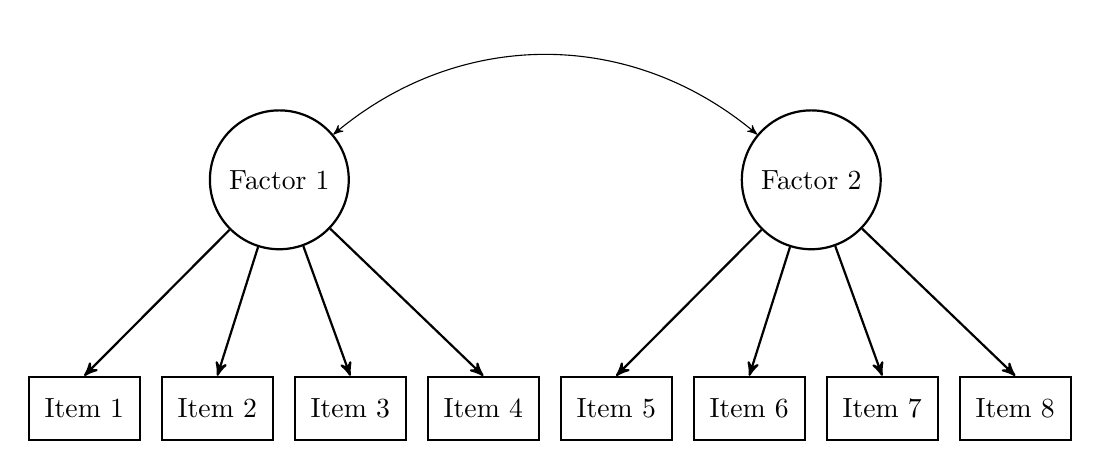
\begin{tikzpicture}[auto,scale=3,
	latent/.style={circle,draw,thick,text badly centered, inner sep=2pt,minimum size=15mm, text width=4.5em, fill=white},
	error/.style={circle,draw,text badly centered, inner sep=2pt,minimum size=10mm},
	manifest/.style={text centered, rectangle,draw,thick,inner sep=3pt,minimum height=8mm, minimum width=10mm, text width= 12mm},
	manifestRot/.style={text centered, rectangle, draw, thick,inner sep=3pt, minimum width=7mm, text width= 7mm, minimum height=15},
	manifestfront/.style={rectangle,draw,thick,inner sep=0pt,minimum size=12mm, fill=white},
	ghost/.style={rectangle, inner sep=0pt,text centered,    minimum height=0mm, minimum width=5mm, text width= 5 mm},
	lcorr/.style={<->,>=stealth', bend right=40},
	rcorr/.style={<->,>=stealth', bend left=40},
	fcorr/.style={<->,>=stealth', bend left=40},
	ofcorr/.style={<->,>=stealth', bend right=60},
	ofcorr2/.style={<->,>=stealth', bend left=60},
	intercept/.style={regular polygon,
        regular polygon sides=3,draw,thick,inner sep=0pt,minimum size=10mm},
	mean/.style={regular polygon,regular polygon sides=3,draw,thick,inner sep=0pt,minimum size=10mm},
	paths/.style={->, thick, >=stealth'},
	variance/.style={<->, thick, >=stealth', bend left=270, looseness=2},
	varianceTop/.style={<->, thick, >=stealth', bend right=270, looseness=2},
	unique/.style={<->, thick, >=stealth', loop below=270, looseness=8},
	factvar/.style={<->, thick, >=stealth', loop right=270, looseness=8}
	] % End Creating Path Model Pieces
\tikzset{mystyle/.style={->,double=black}}


\node [manifest] at (0,0) (x1) {Item 1};
\node [manifest] (x2)  [right = .25cm of x1]  {Item 2};
\node [ghost]    (g1)  [right = 1.5cm of x1]  {};
\node [manifest] (x3)  [right = .25cm of x2]  {Item 3};
\node [manifest] (x4)  [right = .25cm of x3]  {Item 4};

\node [manifest] (x5)  [right = .25cm of x4]  {Item 5};
\node [manifest] (x6)  [right = .25cm of x5]  {Item 6};
\node [ghost]    (g2)  [right = 1.5cm of x5]  {};
\node [manifest] (x7)  [right = .25cm of x6]  {Item 7};
\node [manifest] (x8)  [right = .25cm of x7]  {Item 8};

\node [latent]   (c1)  [above = 2.0cm of g1]  {Factor 1};
\node [latent]   (c2)  [above = 2.0cm of g2]  {Factor 2};

\draw [paths] (c1) to node[pos=0.40, xshift=-5]  {}   (x1.north);
\draw [paths] (c1) to node[pos=0.35, xshift=-3]  {}   (x2.north);
\draw [paths] (c1) to node[pos=0.70, xshift=-3]  {}   (x3.north);
\draw [paths] (c1) to node[pos=0.75, xshift=-7]  {}   (x4.north);

\draw [paths] (c2) to node[pos=0.40, xshift=-5]  {}   (x5.north);
\draw [paths] (c2) to node[pos=0.35, xshift=-3]  {}   (x6.north);
\draw [paths] (c2) to node[pos=0.70, xshift=-3]  {}   (x7.north);
\draw [paths] (c2) to node[pos=0.75, xshift=-7]  {}   (x8.north);


\draw [fcorr] (c1) to node[below] {} (c2);

\end{tikzpicture}
\end{document}